\documentclass[xcolor=dvipsnames]{beamer}

\usepackage{graphicx}
\usepackage{wrapfig}

\mode<presentation>
{
  \usetheme{Warsaw}
  \setbeamercovered{transparent}
}
% \usecolortheme[named=OliveGreen]{structure}
\setbeamertemplate{navigation symbols}{} 
\setbeamertemplate{blocks}[rounded][shadow=true] 

\title{Judy Benjamin and Halpern's \linebreak Full Employment Theory}
\subtitle{Annual Meeting of the Canadian Society \linebreak
  for the History and Philosophy of Science}

\author{Stefan Lukits}

\date{May 29, 2011}

\begin{document}

\begin{frame}
  \titlepage
\end{frame}

\begin{frame}
  \frametitle{Halpern's Full Employment Theorem}
  \begin{columns}
    \column{.50\textwidth}{
Choosing a representation:
    \begin{itemize}
    \item possible worlds
    \item probability measures
    \item lower and upper probabilities
    \item Dempster-Shafer belief functions
    \item possibility measures
    \item ranking functions
    \item relative likelihoods
    \item plausibility measures
    \end{itemize}}
\column{.50\textwidth}{
  \begin{block}{Grove and Halpern}
    ``one must always think carefully about precisely what the
    information means'' \linebreak (``Probability Update \ldots,'' p6)
  \end{block}
  \begin{block}{Joseph Halpern}
    ``there is no escaping the need to understand the details of the
    application'' \linebreak (\emph{Reasoning \ldots}, p423)
  \end{block}
}
  \end{columns}
\end{frame}

\begin{frame}
  \frametitle{Pluralism Versus Statistical Physics I}
  \begin{block}{Statistical Physics}
    ``Jaynes's principle of maximum entropy and Kullbacks
    principle of minimum cross-entropy (minimum directed
    divergence) are shown to be uniquely correct methods for
    inductive inference when new information is given in the form
    of expected values.'' (Shore and Johnson)
  \end{block}
  \begin{block}{Pluralism}
    ``The uniqueness proofs are flawed, or rest on unreasonably
    strong assumptions. A more general class of inference rules,
    maximizing the so-called R{\'e}nyi entropies, is exhibited
    which also fulfill the reasonable part of the consistency
    assumptions.'' (Jos Uffink)
  \end{block}
\end{frame}

\begin{frame}
  \frametitle{Pluralism Versus Statistical Physics II}
  \begin{block}{Statistical Physics}
    ``We show that Skilling's method of induction leads us to a
    unique general theory of inductive inference, the maximum
    entropy method, and precisely how it is that other entropies
    such as those of R{\'e}nyi or Tsallis are ruled out for
    problems of inference. We then explore the compatibility of
    Bayes and maximum entropy updating. We show that maximum
    entropy is capable of producing every aspect of orthodox
    Bayesian inference and prove the complete compatibility of
    Bayesian and entropy methods.'' (Adom Giffin)
 \end{block}
\end{frame}

\begin{frame}
  \frametitle{Pluralism Versus Statistical Physics III}
\begin{block}{Pluralism}
  ``It is perhaps not surprising that there are proponents of maximum
  entropy and relative entropy who recommend that if an agent's
  information can be characterized by a set $C$ of constraints, then
  the agent should act `as if' the probability is determined by the
  measure that maximizes entropy relative to $C$ (i.e., the measure
  that has the highest entropy of all the measures in $C$). Similarly,
  if the agent starts with a particular measure $\mu$ and gets new
  information characterized by $C$, he should update to the measure
  $\mu'$ that satisfies $C$ such that the relative entropy between
  $\mu'$ and $\mu$ is a minimum. Maximum entropy and relative entropy
  have proved quite successful in a number of applications, from
  physics to natural-language modeling. Unfortunately, they also
  exhibit some counterintuitive behavior on certain applications.
  Although they are valuable tools, they should be used with care.''
  \linebreak (Joseph Halpern)
\end{block}
\end{frame}

\begin{frame}
  \frametitle{Objective}
\begin{itemize}
\item[$\rightarrow$] Halpern claims that the principle of maximum entropy
  sometimes exhibits counterintuitive behaviour on certain
  applications. Therefore, the principle of full employment
  applies.
\item[$\rightarrow$] Halpern singles out the Judy Benjamin case to demonstrate
  the counterintuitive behaviour of maximum entropy.
\item[$\rightarrow$] We will show that the Judy Benjamin case does not behave
  counterintuitively when approached via maximum entropy. On the
  contrary, maximum entropy reveals where the information given by
  the case is incompletely specified and provides precisely the
  results that correspond to our intuitions.
\item[$\rightarrow$] Consequently, Halpern does not have a strong case for the
  full employment theory with respect to maximum entropy. This
  supports our larger project of a carefully specified
  epistemological primacy of information theory in matters of
  uncertainty.
\end{itemize}
\end{frame}

\begin{frame}
  \frametitle{The Judy Benjamin Case I}
\begin{figure}[h]
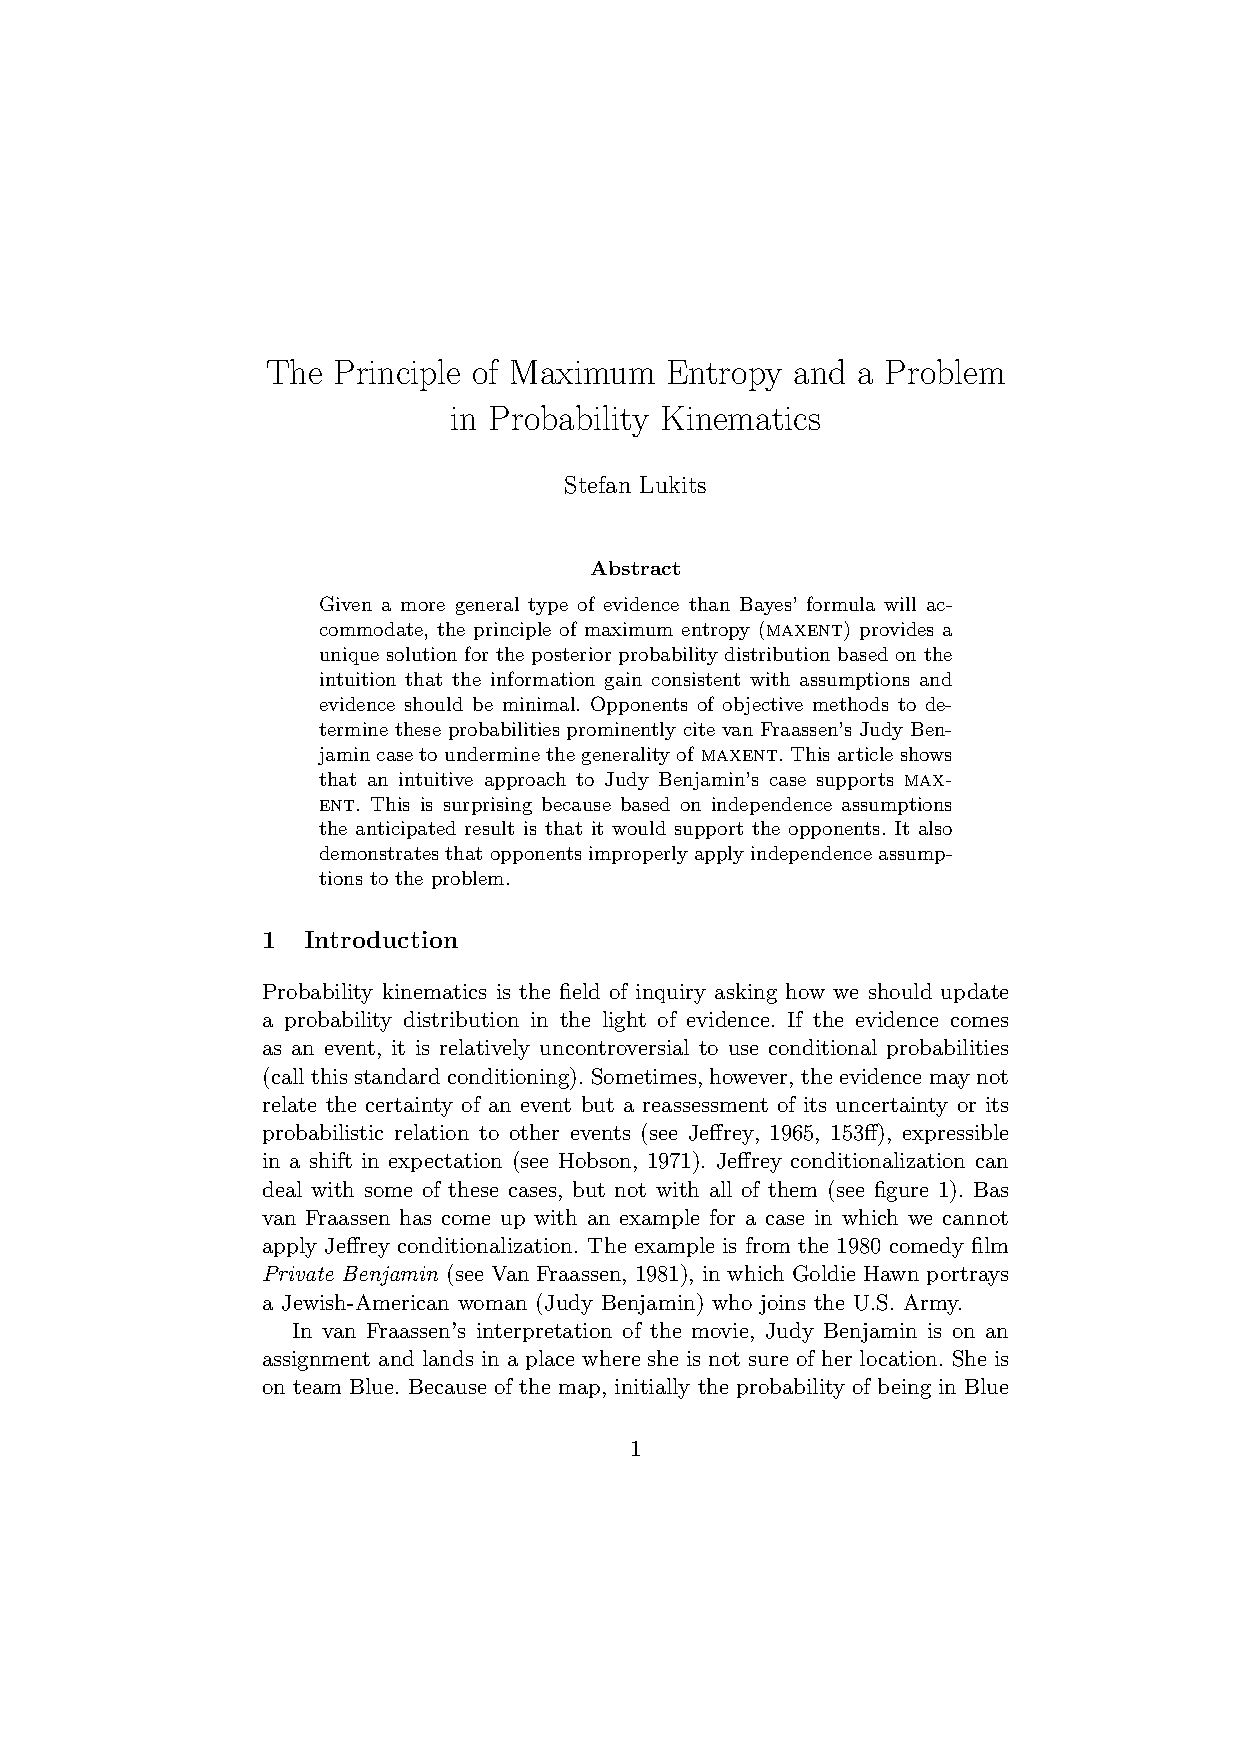
\includegraphics[scale=.5]{judy.pdf}
\end{figure}
\end{frame}

\begin{frame}
  \frametitle{The Judy Benjamin Case II}
\begin{itemize}
\item (MAP) Judy has no idea where she is. She is on team Blue.
  Because of the map, her probability of being in Blue territory
  equals the probability of being in Red territory, and being on Red
  Second Company ground equals the probability of being on Red
  Headquarters ground.
\item (HDQ) Headquarters inform Judy that in case she is in Red
  territory, her chance of being on their Headquarters ground is three
  times the chance of being on their Second Company ground.
\end{itemize}
\begin{equation}
  \label{eq:map}
  2\cdot{}P(A_{1})=2\cdot{}P(A_{2})=P(A_{3})\tag{\mbox{MAP}}
\end{equation}
\begin{equation}
  \label{eq:hdq}
  q=P(A_{2}|A_{1}\cup{}A_{2})=\frac{3}{4}\tag{\mbox{HDQ}}
\end{equation}
\end{frame}

\begin{frame}
  \frametitle{Bayesian Updating}
  \color{blue}{Why Bayesian Updating might not work:}
\begin{itemize}
  \item Bayesian updating requires that an event
    $T\subseteq{}\Omega$ is true.
  \item Sometimes, however, the information received assigns a
    probability to $T$ or a value to the expectation of a random
    variable. We will see that the former case can always be reduced
    to the latter.
  \item Grove and Halpern try to save Bayesian Updating for the
    Judy Benjamin case by setting $T=$``receiving information HDQ.''
  \end{itemize}
\end{frame}

\begin{frame}
  \frametitle{Two Intuitions}
  \begin{itemize}
  \item<1->[\color{blue}{(T1)}] HDQ should not affect $P(A_{3})$. Let's
    call $P$ the prior probability distribution, before receiving HDQ,
    and $Q$ the posterior probability distribution, after receiving
    HDQ. Then $Q(A_{3})=P(A_{3})$.
  \item<2->[\color{blue}{(T2)}] If the value of $q$ approaches $1$
  then $Q(A_{3})$ should approach $2/3$. HDQ would then be ``if you
  are in Red territory you are almost certainly on Red Headquarters
  ground.'' Considering MAP, $Q(A_{3})$ should approach $2/3$.
  Continuity considerations pose a contradiction to T1.
  \end{itemize}
\end{frame}

\begin{frame}
  \frametitle{MAXENT and MINXENT I}
Depending on whether we have a prior probability distribution we can
use \textsc{maxent} or \textsc{minxent} to calculate the posterior
probability distribution using maximum entropy.
\begin{description}
\item[\textsc{maxent}] Choose the probability distribution that
  fulfills the constraint provided by the information you have and is
  otherwise maximally uncertain (maximum entropy).
\item[\textsc{minxent}] Choose the probability distribution that
  fulfills the constraint provided by the information you have and is
  otherwise minimally discriminate from the given prior probability
  distribution (minimum cross-entropy).
\end{description}
\end{frame}

\begin{frame}
  \frametitle{MAXENT and MINXENT II}
  It is most expedient to provide constraints in the form of
  expectations. We define a payoff function $r$ and then set the
  expectation to a value $\alpha$. To be slightly more general, we
  shall call our events $x_{i}$ instead of $A_{i}$, and $m=3$. Let
  $p_{i}=P(A_{i})$ and $q_{i}=Q(A_{i})$.
  \begin{equation}
    \label{eq:map1}
    r(x_{1})=2,r(x_{2})=2,r(x_{3})=0,\alpha=\sum_{i=1}^{m}r(x_{i})q_{i}=1\tag{MAP}
  \end{equation}
  \begin{equation}
    \label{eq:hdq1}
    r(x_{1})=0,r(x_{2})=1,r(x_{3})=q,\alpha=\sum_{i=1}^{m}r(x_{i})q_{i}=q\tag{HDQ}
  \end{equation}
\end{frame}

\begin{frame}
  \frametitle{MAXENT and MINXENT III}
  For \textsc{maxent}, we want to maximize the Shannon entropy:
  \begin{equation}
    \label{eq:maxentfin}
    H(Q)=-\sum_{i=1}^{m}q_{i}\ln{}q_{i}
  \end{equation}
  For \textsc{minxent}, we want to minimize the Kullback-Leibler
  divergence, given first in its general form as a Lebesgue integral
  ($\mu$ is any background measure for which the Radon-Nikodym
  derivatives of $Q$ and $P$ exist), then more applicably to the Judy
  Benjamin case as a finite sum:
  \begin{equation*}
    \label{eq:minxentleb}
    D(Q||P)=\int_{\Omega}q\ln\frac{q}{p}d\mu
  \end{equation*}
  \begin{equation}
    \label{eq:minxentfin}
    D(Q||P)=\sum_{i=1}^{m}q_{i}\ln\frac{q_{i}}{p_{i}}d\mu
  \end{equation}
\end{frame}

\begin{frame}
  \frametitle{The Constraint Rule for \textsc{maxent} I}
Let $f$ be a probability distribution on a finite space
$x_{1},\ldots,x_{m}$ that fulfills the constraint
\begin{equation}
  \label{eq:constraint}
\sum_{i=1}^{m}r(x_{i})f(x_{i})=\alpha
\end{equation}

There are two constraints for $f$:
\begin{equation}
  \label{eq:unity}
\sum_{i=1}^{m}f(x_{i})=1
\end{equation}
\begin{equation}
  \label{eq:entropy}
\mbox{maximize }-\sum_{i=1}^{m}f(x_{i})\ln(x_{i})
\end{equation}
\end{frame}

\begin{frame}
  \frametitle{The Constraint Rule for \textsc{maxent} II}
We use Lagrange multipliers to define the functional
\begin{equation}
  \label{eq:functional}
J(f)=-\sum_{i=1}^{m}f(x_{i})\ln{}f(x_{i})+\lambda_{0}\sum_{i=1}^{m}f+\lambda_{1}\sum_{i=1}^{m}r(x_{1})f(x_{i})
\end{equation}
and differentiate it with respect to $x_{i}$
\begin{equation}
  \label{eq:funder}
\frac{\partial{}J}{\partial{}f(x_{i})}=-\ln(f(x_{i}))-1+\lambda_{0}+\lambda_{1}r(x_{i})
\end{equation}
\end{frame}


\begin{frame}
  \frametitle{The Constraint Rule for \textsc{maxent} III}
Set ({\ref{eq:funder}}) to $0$ to find the necessary condition to
maximize ({\ref{eq:entropy}})
\begin{equation}
  \label{eq:coverthomas}
g(x_{i})=e^{\lambda_{0}-1+\lambda_{1}r(x_{1})}
\end{equation}

This is the Gibbs distribution. We need to (a) show that the entropy
of $g$ is maximal, and (b) show how to find $\lambda_{0}$ and
$\lambda_{1}$. (a) is part of the proof, but we won't need it later
on. We will only show (b). 
\end{frame}

\begin{frame}
  \frametitle{The Constraint Rule for \textsc{maxent} IV}
  Let
  \begin{equation}
  \label{eq:l1}
\lambda_{1}=-\beta
\end{equation}
\begin{equation}
  \label{eq:zet}
Z(\beta)=\sum_{i=1}^{m}e^{-\beta{}r(x_{i})}
\end{equation}
\begin{equation}
  \label{eq:l0}
\lambda_{0}=1-Z(\beta)
\end{equation}

To find $\lambda_{0}$ and $\lambda_{1}$ we set
\begin{equation}
  \label{eq:logcon}
-\frac{\partial}{\partial{}\beta}\ln(Z(\beta))=\alpha
\end{equation}
\end{frame}

\begin{frame}
  \frametitle{The Constraint Rule for \textsc{maxent} V}
  That $g$ so defined maximizes the entropy is shown in (a). We need
  to make sure, however, that with this choice of $\lambda_{0}$ and
  $\lambda_{1}$ the constraints ({\ref{eq:constraint}}) and
  ({\ref{eq:unity}}) are also fulfilled.

  First, we show
  \begin{align}
    &\sum_{i=1}^{m}g(x_{i})=\sum_{i=1}^{m}e^{\lambda_{0}-1+\lambda_{1}r(x_{i})}=e^{\lambda_{0}}\sum_{i=1}^{m}e^{\lambda_{1}r(x_{i})}=\notag\\
    &e^{-\ln(Z(\beta))}Z(\beta)=1\label{eq:unishow}
  \end{align}
\end{frame}

\begin{frame}
  \frametitle{The Constraint Rule for \textsc{maxent} VI}
  Then, we show, by differentiating $\ln(Z(\beta))$ using the
  substitution $x=e^{-\beta}$
  \begin{align}
    &\alpha=-\frac{\partial}{\partial{}\beta}\ln(Z(\beta))=-\frac{1}{\sum_{i=1}^{m}x^{r(x_{i})}}\left(\sum_{i=1}^{m}r(x_{i})x^{r(x_{i})-1}\right)(-x)=\notag\\
    &\frac{\sum_{i=1}^{m}r(x_{i})x^{r(x_{i})}}{\sum_{i=1}^{m}x^{r(x_{i})}}\label{eq:alphashow}
  \end{align}

  And, finally,
  \begin{align}
    &\sum_{i=1}^{m}r(x_{i})g(x_{i})=\sum_{i=1}^{m}r(x_{i})e^{\lambda_{0}-1+\lambda_{1}r(x_{1})}=e^{\lambda_{0}-1}\sum_{i=1}^{m}r(x_{i})e^{\lambda_{1}r(x_{1})}=\notag\\
    &e^{\lambda_{0}-1}\sum_{i=1}^{m}r(x_{i})x^{r(x_{i})}=\alpha{}e^{\lambda_{0}-1}\sum_{i=1}^{m}x^{r(x_{i})}=\alpha{}e^{\lambda_{0}-1}\sum_{i=1}^{m}e^{-\beta{}r(x_{i})}=\notag\\
    &\alpha{}Z(\beta)e^{\lambda_{0}-1}=\alpha{}Z(\beta))e^{-\ln(Z(\beta))}=\alpha\label{eq:finalshow}
  \end{align}
\end{frame}

\begin{frame}
  \frametitle{The Constraint Rule Applied to Judy Benjamin I}
  The normalized odds vector for the Judy Benjamin case without using
  information ({\ref{eq:hdq}}) is:
  \begin{displaymath}
    v_{0}=(.25,.25,.5)
  \end{displaymath}

  Let's apply the constraint rule to the Judy Benjamin case. Instead
  of proving an analogous procedure for \textsc{minxent}, we first
  calculate the posterior using the information for ({\ref{eq:hdq}}),
  but not yet for ({\ref{eq:map}}), so that we can use the procedure
  for \textsc{maxent} that we just spelled out.
  ({\ref{eq:constraint}}) is defined by ({\ref{eq:hdq1}}). The lambdas
  are:
  \begin{align}
    &\lambda_{0}=1-\ln\left(\sum_{i=1}^{m}e^{\lambda_{1}r(x_{i})}\right)\notag
    &\lambda_{1}=\ln{}q-\ln(1-q)\notag
  \end{align}
\end{frame}

\begin{frame}
  \frametitle{The Constraint Rule Applied to Judy Benjamin II}
  We combine the normalized odds vector following from these lambdas
  ($v_{2}=(.16,.48,.36)$) using Dempster's Rule of Combination with
  ({\ref{eq:map}}) and get
  \begin{displaymath}
    v_{1}=(.12,.35,.53)
  \end{displaymath}

  You can check this result by differentiating and examining the
  critical points of the Kullback-Leibler divergence directly (see
  next slide). It contradicts intuition (T1) because $q_{3}=.53$ is no
  longer 1/2.
\end{frame}

\begin{frame}
  \frametitle{$q_{1}$ as a Function of $q$}
  Differentiating and examining the critical points of the
  Kullback-Leibler divergence directly gives us the following function
  $q\rightarrow{}q_{1}$:
  \begin{displaymath}
q_{1}=\frac{s}{1+st+s}
\end{displaymath}
  \begin{align}
& s=2^{-\frac{t\log_{2}t+t+1}{t+1}}\notag
& t=\frac{q}{q-1}\notag
  \end{align}
\end{frame}

\begin{frame}
  \frametitle{Intuition (T2)}
  \begin{figure}[h]
    \includegraphics[scale=.4]{plot-i2.jpg}
  \end{figure}
\end{frame}

\begin{frame}
  \frametitle{Intuition (T1)}
  \begin{figure}[h]
    \includegraphics[scale=.4]{plot-i1.jpg}
  \end{figure}
\end{frame}

\begin{frame}
  \frametitle{Four Scenarios I}
  Here are four scenarios, in which Judy may have received
  ({\ref{eq:hdq}}):
\begin{enumerate}
\item[S1] Judy was dropped off by a pilot who flipped two coins. If
  the first coin landed H, then Judy was dropped off in Blue
  territory, otherwise in Red territory. If the second coin landed H,
  she was dropped off on Headquarters ground, otherwise on Second
  Company ground. Judy's headquarters find out that the second coin
  was biased $q:1-q$ toward H. The normalized odds vector is
  $v=(.125,.375,.5)$ and agrees with (T1), because the choice of Blue
  or Red is completely independent from the choice of Headquarters or
  Second Company.
\end{enumerate}
\end{frame}

\begin{frame}
  \frametitle{Four Scenarios II}
\begin{enumerate}
\item [S2] Judy's Headquarters has divided the map into $24$ congruent
  rectangles, $A_{3}$ into twelve, and $A_{1}$ and $A_{2}$ into six
  rectangles each. They have information that the only subsets of the
  $24$ rectangles in which Judy Benjamin may be located are such that
  they contain three times as many $A_{2}$ rectangles than $A_{1}$
  rectangles. Thus they relay ({\ref{eq:hdq}}) to Judy, which she
  correctly interprets with the normalized odds vector
  $v=(.108,.324,.568)$ (evaluating the $16777216$ subsets).
\end{enumerate}
\end{frame}

\begin{frame}
  \frametitle{Four Scenarios III-IV}
\begin{enumerate}
\item[S3] The pilot randomly lands in any of the four quadrants and
  rolls a die. If she rolls an even number, she drops off Judy. If
  not, she takes her to another (or the same) randomly selected
  quadrant to repeat the procedure. Headquarters find out, however,
  that for $A_{1}$, the pilot requires a six to drop off Judy, not
  just an even number. Thus they relay ({\ref{eq:hdq}}) to Judy, which
  she correctly interprets with the normalized odds vector
  $v=(.1,.3,.6)$.
\item [S4] Judy's headquarters know that Judy is not in $A_{3}$ and
  that her chance of being in $A_{2}$ is three times the chance of
  being in $A_{1}$. They only succeed, however, in informing Judy of
  the second part of the message. If Judy had all the information, her
  normalized odds vector would be $v=(.33,.67,0)$.
\end{enumerate}
\end{frame}

\begin{frame}
  \frametitle{Knowledge Expands Ignorance}
  In short, given only ({\ref{eq:map}}) and ({\ref{eq:hdq}}), Judy
  cannot have any confidence that they are independent. Consequently,
  she should adjust her probabilities using $v_{1}$ in accordance with
  (T2). Van Fraassen is worried that she has now greater confidence in
  being in Blue territory, without receiving any specific information
  about it. As so often, there is discomfort with the ability of
  maximum entropy to articulate a hypothesis on the basis of ignorance
  rather than positive evidence. It may be intuitive that an increase
  in knowledge and certainty about part of the event space also
  increases the posterior probability of the space about which we are
  ignorant.
\end{frame}

\begin{frame}
  \frametitle{End of Presentation}
\end{frame}

\end{document}